\documentclass[twoside]{book}

% Packages required by doxygen
\usepackage{fixltx2e}
\usepackage{calc}
\usepackage{doxygen}
\usepackage[export]{adjustbox} % also loads graphicx
\usepackage{graphicx}
\usepackage[utf8]{inputenc}
\usepackage{makeidx}
\usepackage{multicol}
\usepackage{multirow}
\PassOptionsToPackage{warn}{textcomp}
\usepackage{textcomp}
\usepackage[nointegrals]{wasysym}
\usepackage[table]{xcolor}

% Font selection
\usepackage[T1]{fontenc}
\usepackage[scaled=.90]{helvet}
\usepackage{courier}
\usepackage{amssymb}
\usepackage{sectsty}
\renewcommand{\familydefault}{\sfdefault}
\allsectionsfont{%
  \fontseries{bc}\selectfont%
  \color{darkgray}%
}
\renewcommand{\DoxyLabelFont}{%
  \fontseries{bc}\selectfont%
  \color{darkgray}%
}
\newcommand{\+}{\discretionary{\mbox{\scriptsize$\hookleftarrow$}}{}{}}

% Page & text layout
\usepackage{geometry}
\geometry{%
  a4paper,%
  top=2.5cm,%
  bottom=2.5cm,%
  left=2.5cm,%
  right=2.5cm%
}
\tolerance=750
\hfuzz=15pt
\hbadness=750
\setlength{\emergencystretch}{15pt}
\setlength{\parindent}{0cm}
\setlength{\parskip}{3ex plus 2ex minus 2ex}
\makeatletter
\renewcommand{\paragraph}{%
  \@startsection{paragraph}{4}{0ex}{-1.0ex}{1.0ex}{%
    \normalfont\normalsize\bfseries\SS@parafont%
  }%
}
\renewcommand{\subparagraph}{%
  \@startsection{subparagraph}{5}{0ex}{-1.0ex}{1.0ex}{%
    \normalfont\normalsize\bfseries\SS@subparafont%
  }%
}
\makeatother

% Headers & footers
\usepackage{fancyhdr}
\pagestyle{fancyplain}
\fancyhead[LE]{\fancyplain{}{\bfseries\thepage}}
\fancyhead[CE]{\fancyplain{}{}}
\fancyhead[RE]{\fancyplain{}{\bfseries\leftmark}}
\fancyhead[LO]{\fancyplain{}{\bfseries\rightmark}}
\fancyhead[CO]{\fancyplain{}{}}
\fancyhead[RO]{\fancyplain{}{\bfseries\thepage}}
\fancyfoot[LE]{\fancyplain{}{}}
\fancyfoot[CE]{\fancyplain{}{}}
\fancyfoot[RE]{\fancyplain{}{\bfseries\scriptsize Generated by Doxygen }}
\fancyfoot[LO]{\fancyplain{}{\bfseries\scriptsize Generated by Doxygen }}
\fancyfoot[CO]{\fancyplain{}{}}
\fancyfoot[RO]{\fancyplain{}{}}
\renewcommand{\footrulewidth}{0.4pt}
\renewcommand{\chaptermark}[1]{%
  \markboth{#1}{}%
}
\renewcommand{\sectionmark}[1]{%
  \markright{\thesection\ #1}%
}

% Indices & bibliography
\usepackage{natbib}
\usepackage[titles]{tocloft}
\setcounter{tocdepth}{3}
\setcounter{secnumdepth}{5}
\makeindex

% Hyperlinks (required, but should be loaded last)
\usepackage{ifpdf}
\ifpdf
  \usepackage[pdftex,pagebackref=true]{hyperref}
\else
  \usepackage[ps2pdf,pagebackref=true]{hyperref}
\fi
\hypersetup{%
  colorlinks=true,%
  linkcolor=blue,%
  citecolor=blue,%
  unicode%
}

% Custom commands
\newcommand{\clearemptydoublepage}{%
  \newpage{\pagestyle{empty}\cleardoublepage}%
}

\usepackage{caption}
\captionsetup{labelsep=space,justification=centering,font={bf},singlelinecheck=off,skip=4pt,position=top}

%===== C O N T E N T S =====

\begin{document}

% Titlepage & ToC
\hypersetup{pageanchor=false,
             bookmarksnumbered=true,
             pdfencoding=unicode
            }
\pagenumbering{alph}
\begin{titlepage}
\vspace*{7cm}
\begin{center}%
{\Large Decorator }\\
\vspace*{1cm}
{\large Generated by Doxygen 1.8.13}\\
\end{center}
\end{titlepage}
\clearemptydoublepage
\pagenumbering{roman}
\tableofcontents
\clearemptydoublepage
\pagenumbering{arabic}
\hypersetup{pageanchor=true}

%--- Begin generated contents ---
\chapter{Namespace Index}
\section{Packages}
Here are the packages with brief descriptions (if available)\+:\begin{DoxyCompactList}
\item\contentsline{section}{\hyperlink{namespace_decorator}{Decorator} }{\pageref{namespace_decorator}}{}
\end{DoxyCompactList}

\chapter{Hierarchical Index}
\section{Class Hierarchy}
This inheritance list is sorted roughly, but not completely, alphabetically\+:\begin{DoxyCompactList}
\item \contentsline{section}{Strategy.\+Dojazd}{\pageref{interface_strategy_1_1_dojazd}}{}
\begin{DoxyCompactList}
\item \contentsline{section}{Strategy.\+Rower}{\pageref{class_strategy_1_1_rower}}{}
\item \contentsline{section}{Strategy.\+Samochod}{\pageref{class_strategy_1_1_samochod}}{}
\end{DoxyCompactList}
\item \contentsline{section}{Strategy.\+Praca}{\pageref{interface_strategy_1_1_praca}}{}
\begin{DoxyCompactList}
\item \contentsline{section}{Strategy.\+Maluje\+Samochod}{\pageref{class_strategy_1_1_maluje_samochod}}{}
\item \contentsline{section}{Strategy.\+Montuje\+Silnik}{\pageref{class_strategy_1_1_montuje_silnik}}{}
\item \contentsline{section}{Strategy.\+Testuje\+Samochodow}{\pageref{class_strategy_1_1_testuje_samochodow}}{}
\end{DoxyCompactList}
\item \contentsline{section}{Strategy.\+Pracownik}{\pageref{class_strategy_1_1_pracownik}}{}
\item \contentsline{section}{Strategy.\+Spedzanie\+Wolnego\+Czasu}{\pageref{interface_strategy_1_1_spedzanie_wolnego_czasu}}{}
\begin{DoxyCompactList}
\item \contentsline{section}{Strategy.\+Gra\+Komputerowa}{\pageref{class_strategy_1_1_gra_komputerowa}}{}
\item \contentsline{section}{Strategy.\+Literatura\+Popularno\+Naukowa}{\pageref{class_strategy_1_1_literatura_popularno_naukowa}}{}
\item \contentsline{section}{Strategy.\+Silownia}{\pageref{class_strategy_1_1_silownia}}{}
\end{DoxyCompactList}
\item \contentsline{section}{Strategy.\+Strategy}{\pageref{class_strategy_1_1_strategy}}{}
\end{DoxyCompactList}

\chapter{Class Index}
\section{Class List}
Here are the classes, structs, unions and interfaces with brief descriptions\+:\begin{DoxyCompactList}
\item\contentsline{section}{\hyperlink{class_lazy_1_1_custom_lazy_class}{Lazy.\+Custom\+Lazy\+Class} \\*\hyperlink{class_lazy_1_1_custom_lazy_class}{Custom\+Lazy\+Class} posiada zmienna \+\_\+\+Value inicjalizowaną tuż przed uzyciem }{\pageref{class_lazy_1_1_custom_lazy_class}}{}
\item\contentsline{section}{\hyperlink{class_lazy_1_1_lazy}{Lazy.\+Lazy} \\*Klasa zawierająca funkcje Main }{\pageref{class_lazy_1_1_lazy}}{}
\item\contentsline{section}{\hyperlink{class_lazy_1_1_lazy_class}{Lazy.\+Lazy\+Class} \\*\hyperlink{class_lazy_1_1_lazy_class}{Lazy\+Class} posiada zmienna Value }{\pageref{class_lazy_1_1_lazy_class}}{}
\end{DoxyCompactList}

\chapter{Namespace Documentation}
\hypertarget{namespace_decorator}{}\section{Decorator Namespace Reference}
\label{namespace_decorator}\index{Decorator@{Decorator}}
\subsection*{Classes}
\begin{DoxyCompactItemize}
\item 
class \hyperlink{class_decorator_1_1_decorator}{Decorator}
\begin{DoxyCompactList}\small\item\em Klasa zawierająca funkcje Main \end{DoxyCompactList}\item 
class \hyperlink{class_decorator_1_1_dekorator}{Dekorator}
\begin{DoxyCompactList}\small\item\em \hyperlink{class_decorator_1_1_dekorator}{Dekorator} dla obiektu \hyperlink{class_decorator_1_1_samochod}{Samochod} \end{DoxyCompactList}\item 
class \hyperlink{class_decorator_1_1_ford}{Ford}
\begin{DoxyCompactList}\small\item\em Klasa dziedziczaca z \hyperlink{class_decorator_1_1_samochod}{Samochod} \end{DoxyCompactList}\item 
class \hyperlink{class_decorator_1_1_klimatyzacja}{Klimatyzacja}
\begin{DoxyCompactList}\small\item\em Klasa dziedziczaca z \hyperlink{class_decorator_1_1_dekorator}{Dekorator} \end{DoxyCompactList}\item 
class \hyperlink{class_decorator_1_1_mercedes}{Mercedes}
\begin{DoxyCompactList}\small\item\em Klasa dziedziczaca z \hyperlink{class_decorator_1_1_samochod}{Samochod} \end{DoxyCompactList}\item 
class \hyperlink{class_decorator_1_1_opony_zimowe}{Opony\+Zimowe}
\begin{DoxyCompactList}\small\item\em Klasa dziedziczaca z \hyperlink{class_decorator_1_1_dekorator}{Dekorator} \end{DoxyCompactList}\item 
class \hyperlink{class_decorator_1_1_samochod}{Samochod}
\begin{DoxyCompactList}\small\item\em Podstawowy obiekt, nieudekorowany \end{DoxyCompactList}\end{DoxyCompactItemize}

\chapter{Class Documentation}
\hypertarget{class_decorator_1_1_decorator}{}\section{Decorator.\+Decorator Class Reference}
\label{class_decorator_1_1_decorator}\index{Decorator.\+Decorator@{Decorator.\+Decorator}}


Klasa zawierająca funkcje Main  


\subsection*{Static Public Member Functions}
\begin{DoxyCompactItemize}
\item 
\mbox{\Hypertarget{class_decorator_1_1_decorator_af259ab736aee14120bdfdb90e64246c6}\label{class_decorator_1_1_decorator_af259ab736aee14120bdfdb90e64246c6}} 
static void {\bfseries Main} (String\mbox{[}$\,$\mbox{]} args)
\end{DoxyCompactItemize}


\subsection{Detailed Description}
Klasa zawierająca funkcje Main 



The documentation for this class was generated from the following file\+:\begin{DoxyCompactItemize}
\item 
Program.\+cs\end{DoxyCompactItemize}

\hypertarget{class_decorator_1_1_dekorator}{}\section{Decorator.\+Dekorator Class Reference}
\label{class_decorator_1_1_dekorator}\index{Decorator.\+Dekorator@{Decorator.\+Dekorator}}


\hyperlink{class_decorator_1_1_dekorator}{Dekorator} dla obiektu \hyperlink{class_decorator_1_1_samochod}{Samochod}  


Inheritance diagram for Decorator.\+Dekorator\+:\begin{figure}[H]
\begin{center}
\leavevmode
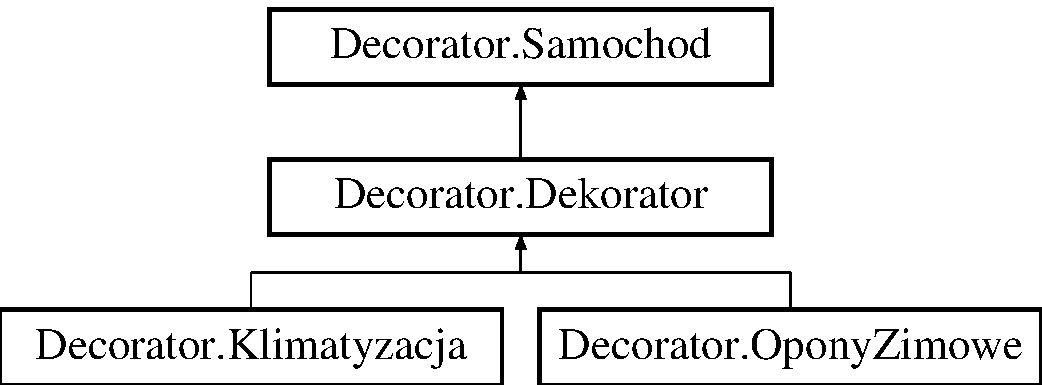
\includegraphics[height=3.000000cm]{class_decorator_1_1_dekorator}
\end{center}
\end{figure}
\subsection*{Public Member Functions}
\begin{DoxyCompactItemize}
\item 
\mbox{\Hypertarget{class_decorator_1_1_dekorator_a49bedb3447feedd5c1595ed048747756}\label{class_decorator_1_1_dekorator_a49bedb3447feedd5c1595ed048747756}} 
abstract override String {\bfseries about} ()
\end{DoxyCompactItemize}
\subsection*{Additional Inherited Members}


\subsection{Detailed Description}
\hyperlink{class_decorator_1_1_dekorator}{Dekorator} dla obiektu \hyperlink{class_decorator_1_1_samochod}{Samochod} 



The documentation for this class was generated from the following file\+:\begin{DoxyCompactItemize}
\item 
Program.\+cs\end{DoxyCompactItemize}

\hypertarget{class_decorator_1_1_ford}{}\section{Decorator.\+Ford Class Reference}
\label{class_decorator_1_1_ford}\index{Decorator.\+Ford@{Decorator.\+Ford}}


Klasa dziedziczaca z \hyperlink{class_decorator_1_1_samochod}{Samochod}  


Inheritance diagram for Decorator.\+Ford\+:\begin{figure}[H]
\begin{center}
\leavevmode
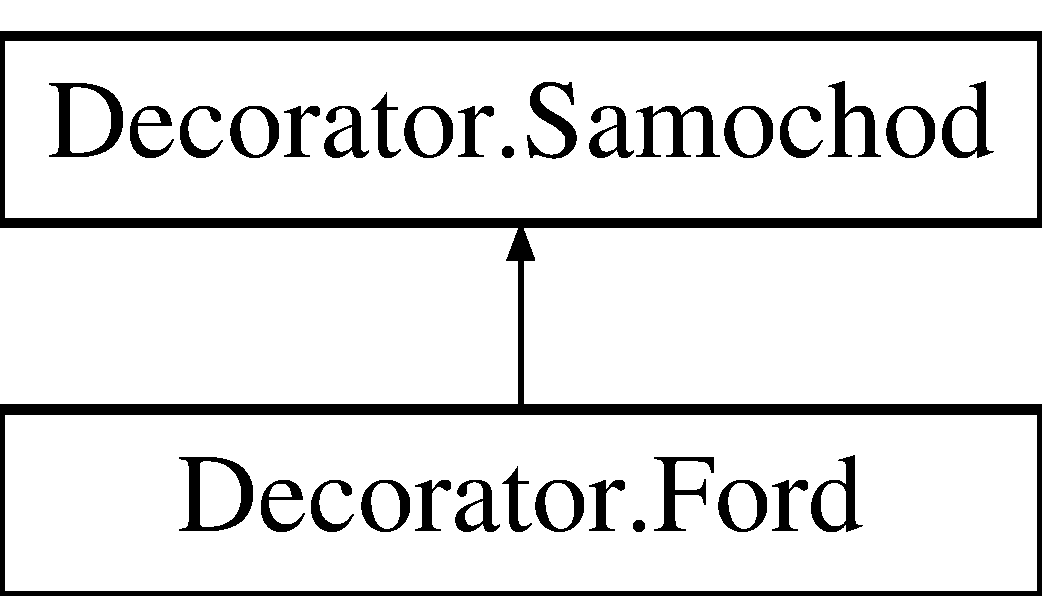
\includegraphics[height=2.000000cm]{class_decorator_1_1_ford}
\end{center}
\end{figure}
\subsection*{Public Member Functions}
\begin{DoxyCompactItemize}
\item 
\mbox{\Hypertarget{class_decorator_1_1_ford_af514c0d0a73eb596258f1ba23d613d30}\label{class_decorator_1_1_ford_af514c0d0a73eb596258f1ba23d613d30}} 
override double {\bfseries cena} ()
\end{DoxyCompactItemize}
\subsection*{Additional Inherited Members}


\subsection{Detailed Description}
Klasa dziedziczaca z \hyperlink{class_decorator_1_1_samochod}{Samochod} 



The documentation for this class was generated from the following file\+:\begin{DoxyCompactItemize}
\item 
Program.\+cs\end{DoxyCompactItemize}

\hypertarget{class_decorator_1_1_klimatyzacja}{}\section{Decorator.\+Klimatyzacja Class Reference}
\label{class_decorator_1_1_klimatyzacja}\index{Decorator.\+Klimatyzacja@{Decorator.\+Klimatyzacja}}


Klasa dziedziczaca z \hyperlink{class_decorator_1_1_dekorator}{Dekorator}  


Inheritance diagram for Decorator.\+Klimatyzacja\+:\begin{figure}[H]
\begin{center}
\leavevmode
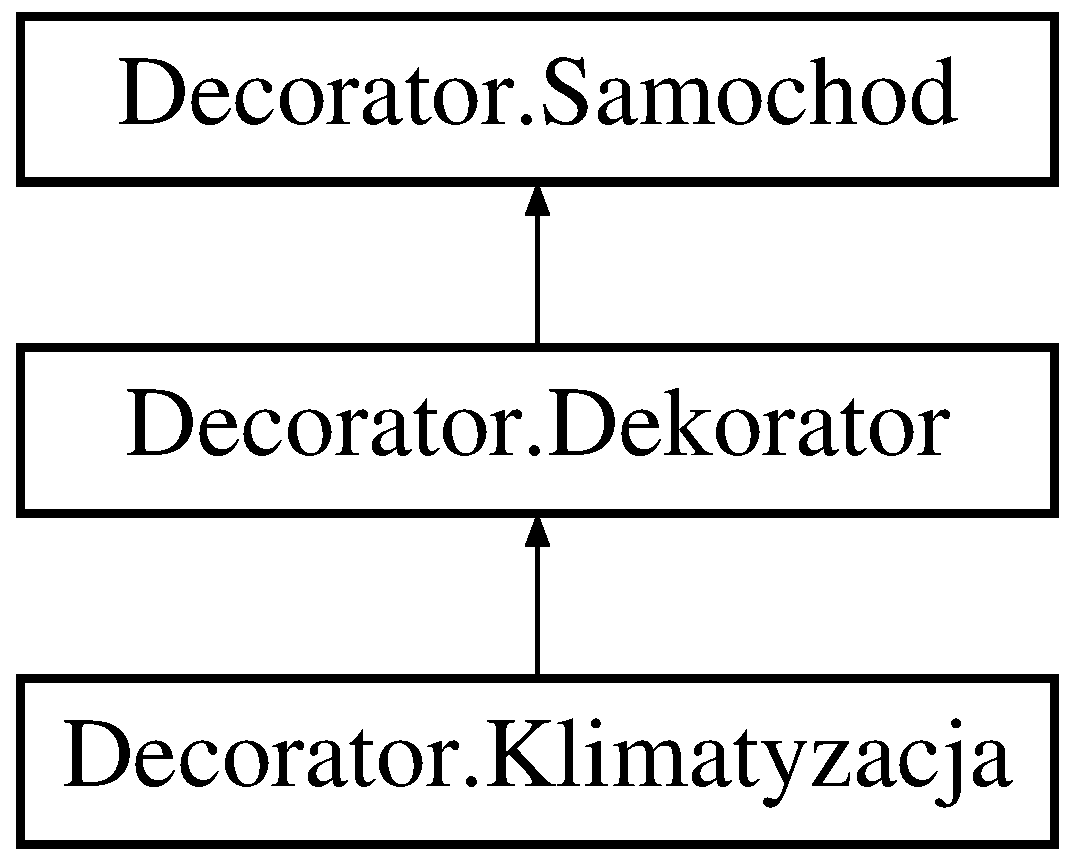
\includegraphics[height=3.000000cm]{class_decorator_1_1_klimatyzacja}
\end{center}
\end{figure}
\subsection*{Public Member Functions}
\begin{DoxyCompactItemize}
\item 
\mbox{\Hypertarget{class_decorator_1_1_klimatyzacja_aeb6393dfcaddcaeac296e873824e5f7d}\label{class_decorator_1_1_klimatyzacja_aeb6393dfcaddcaeac296e873824e5f7d}} 
{\bfseries Klimatyzacja} (\hyperlink{class_decorator_1_1_samochod}{Samochod} samochod)
\item 
\mbox{\Hypertarget{class_decorator_1_1_klimatyzacja_a0f8564f1298a5d410506a3ea87bad970}\label{class_decorator_1_1_klimatyzacja_a0f8564f1298a5d410506a3ea87bad970}} 
override String {\bfseries about} ()
\item 
\mbox{\Hypertarget{class_decorator_1_1_klimatyzacja_ac94c3f63d29ed8edff7e41053f01adda}\label{class_decorator_1_1_klimatyzacja_ac94c3f63d29ed8edff7e41053f01adda}} 
override double {\bfseries cena} ()
\end{DoxyCompactItemize}
\subsection*{Additional Inherited Members}


\subsection{Detailed Description}
Klasa dziedziczaca z \hyperlink{class_decorator_1_1_dekorator}{Dekorator} 



The documentation for this class was generated from the following file\+:\begin{DoxyCompactItemize}
\item 
Program.\+cs\end{DoxyCompactItemize}

\hypertarget{class_decorator_1_1_mercedes}{}\section{Decorator.\+Mercedes Class Reference}
\label{class_decorator_1_1_mercedes}\index{Decorator.\+Mercedes@{Decorator.\+Mercedes}}


Klasa dziedziczaca z \hyperlink{class_decorator_1_1_samochod}{Samochod}  


Inheritance diagram for Decorator.\+Mercedes\+:\begin{figure}[H]
\begin{center}
\leavevmode
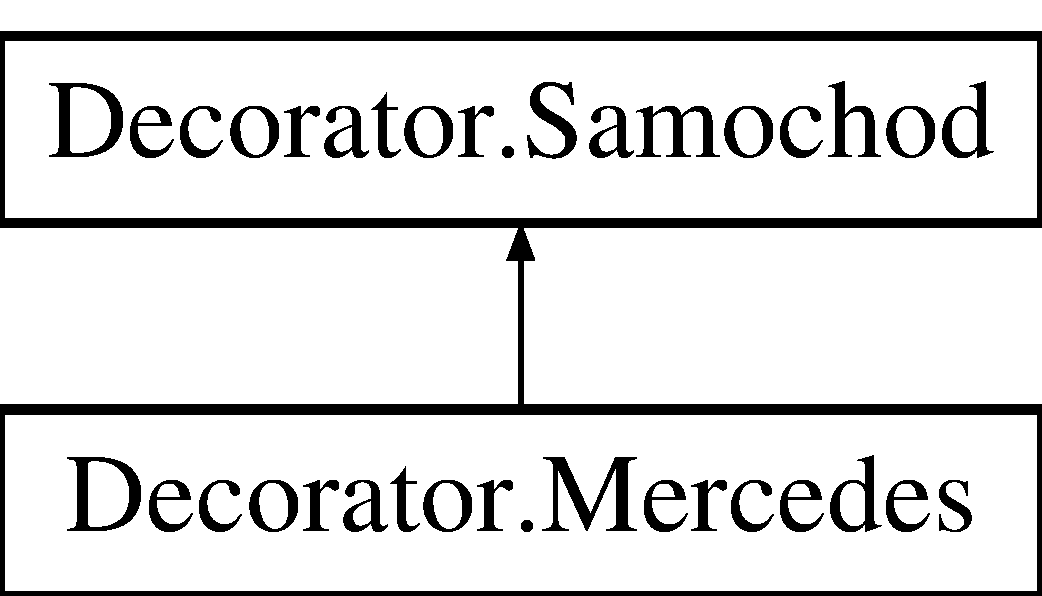
\includegraphics[height=2.000000cm]{class_decorator_1_1_mercedes}
\end{center}
\end{figure}
\subsection*{Public Member Functions}
\begin{DoxyCompactItemize}
\item 
\mbox{\Hypertarget{class_decorator_1_1_mercedes_a86a532d19bd7b691e504d1dee0aee529}\label{class_decorator_1_1_mercedes_a86a532d19bd7b691e504d1dee0aee529}} 
override double {\bfseries cena} ()
\end{DoxyCompactItemize}
\subsection*{Additional Inherited Members}


\subsection{Detailed Description}
Klasa dziedziczaca z \hyperlink{class_decorator_1_1_samochod}{Samochod} 



The documentation for this class was generated from the following file\+:\begin{DoxyCompactItemize}
\item 
Program.\+cs\end{DoxyCompactItemize}

\hypertarget{class_decorator_1_1_opony_zimowe}{}\section{Decorator.\+Opony\+Zimowe Class Reference}
\label{class_decorator_1_1_opony_zimowe}\index{Decorator.\+Opony\+Zimowe@{Decorator.\+Opony\+Zimowe}}


Klasa dziedziczaca z \hyperlink{class_decorator_1_1_dekorator}{Dekorator}  


Inheritance diagram for Decorator.\+Opony\+Zimowe\+:\begin{figure}[H]
\begin{center}
\leavevmode
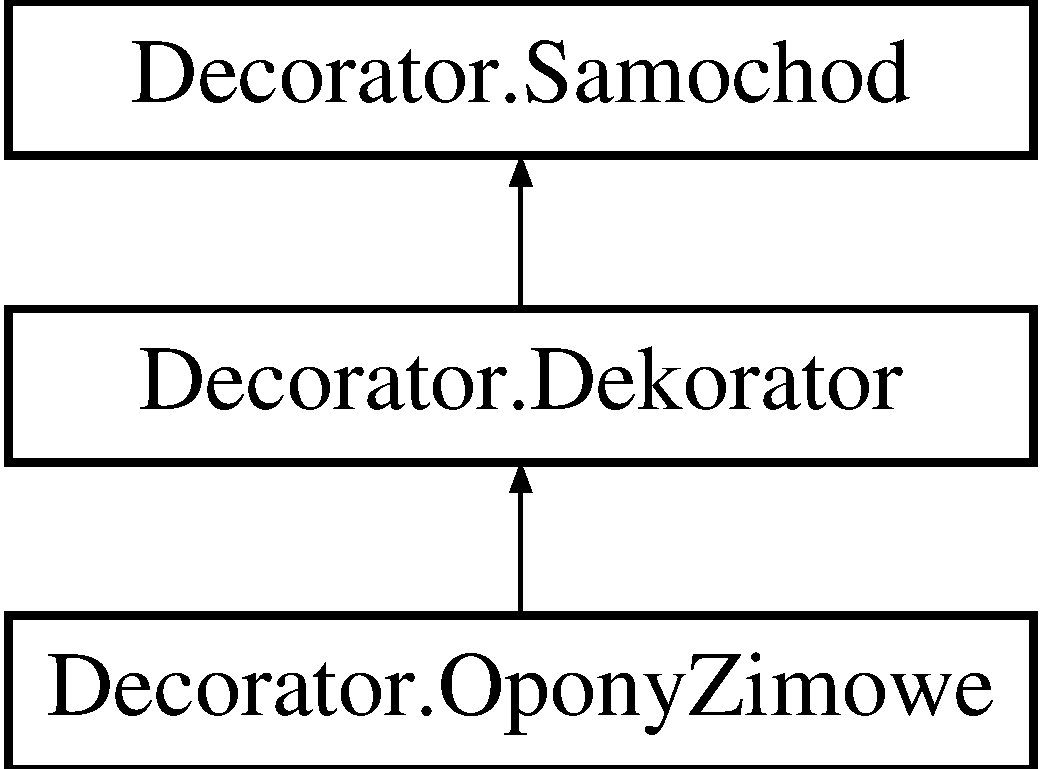
\includegraphics[height=3.000000cm]{class_decorator_1_1_opony_zimowe}
\end{center}
\end{figure}
\subsection*{Public Member Functions}
\begin{DoxyCompactItemize}
\item 
\mbox{\Hypertarget{class_decorator_1_1_opony_zimowe_aa3e242dd62668d4c803d22ab7371ebcc}\label{class_decorator_1_1_opony_zimowe_aa3e242dd62668d4c803d22ab7371ebcc}} 
{\bfseries Opony\+Zimowe} (\hyperlink{class_decorator_1_1_samochod}{Samochod} samochod)
\item 
\mbox{\Hypertarget{class_decorator_1_1_opony_zimowe_aa4aef4edfce638b708e069eb23787e99}\label{class_decorator_1_1_opony_zimowe_aa4aef4edfce638b708e069eb23787e99}} 
override String {\bfseries about} ()
\item 
\mbox{\Hypertarget{class_decorator_1_1_opony_zimowe_a2fc76a06de0b8a57aa908cc4e589e861}\label{class_decorator_1_1_opony_zimowe_a2fc76a06de0b8a57aa908cc4e589e861}} 
override double {\bfseries cena} ()
\end{DoxyCompactItemize}
\subsection*{Additional Inherited Members}


\subsection{Detailed Description}
Klasa dziedziczaca z \hyperlink{class_decorator_1_1_dekorator}{Dekorator} 



The documentation for this class was generated from the following file\+:\begin{DoxyCompactItemize}
\item 
Program.\+cs\end{DoxyCompactItemize}

\hypertarget{class_decorator_1_1_samochod}{}\section{Decorator.\+Samochod Class Reference}
\label{class_decorator_1_1_samochod}\index{Decorator.\+Samochod@{Decorator.\+Samochod}}


Podstawowy obiekt, nieudekorowany  


Inheritance diagram for Decorator.\+Samochod\+:\begin{figure}[H]
\begin{center}
\leavevmode
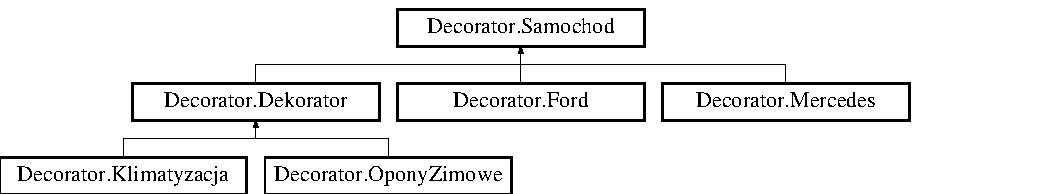
\includegraphics[height=2.576687cm]{class_decorator_1_1_samochod}
\end{center}
\end{figure}
\subsection*{Public Member Functions}
\begin{DoxyCompactItemize}
\item 
\mbox{\Hypertarget{class_decorator_1_1_samochod_a48c5591c5ee338bfe4c1c5c7d26fde8d}\label{class_decorator_1_1_samochod_a48c5591c5ee338bfe4c1c5c7d26fde8d}} 
virtual String {\bfseries about} ()
\item 
\mbox{\Hypertarget{class_decorator_1_1_samochod_a1e2150121674454a06f3f6ec7092d134}\label{class_decorator_1_1_samochod_a1e2150121674454a06f3f6ec7092d134}} 
abstract double {\bfseries cena} ()
\end{DoxyCompactItemize}
\subsection*{Protected Attributes}
\begin{DoxyCompactItemize}
\item 
\mbox{\Hypertarget{class_decorator_1_1_samochod_a4493a233669270a561f60916f52f7f2e}\label{class_decorator_1_1_samochod_a4493a233669270a561f60916f52f7f2e}} 
string {\bfseries samochod} = \char`\"{}Samochod podstawowy\char`\"{}
\end{DoxyCompactItemize}


\subsection{Detailed Description}
Podstawowy obiekt, nieudekorowany 



The documentation for this class was generated from the following file\+:\begin{DoxyCompactItemize}
\item 
Program.\+cs\end{DoxyCompactItemize}

%--- End generated contents ---

% Index
\backmatter
\newpage
\phantomsection
\clearemptydoublepage
\addcontentsline{toc}{chapter}{Index}
\printindex

\end{document}
